\documentclass[12pt,a4paper]{article}
\usepackage[utf8]{inputenc}
\usepackage[vietnamese]{babel}
\usepackage{graphicx}
\usepackage{float}
\usepackage{geometry}
\geometry{a4paper, margin=2cm}
\usepackage{hyperref}
\usepackage{xcolor}
\usepackage{fancyhdr}
\usepackage{titlesec}
\usepackage{booktabs}
\usepackage{array}
\usepackage{amssymb} % để dùng kí hiệu ngôi sao hoặc biểu tượng khác

\hypersetup{
    colorlinks=true,
    linkcolor=blue,
    filecolor=magenta,      
    urlcolor=cyan,
    pdftitle={Bao cao Bai tap 2 - Danh gia thong tin hoc thuat},
    pdfpagemode=FullScreen,
}

% Cấu hình header & footer
\pagestyle{fancy}
\fancyhf{}
\rhead{Hành trình Kỹ năng số}
\lhead{Bài tập Thực hành 2}
\rfoot{Trang \thepage}

% Định dạng tiêu đề mục
\titleformat{\section}{\normalfont\Large\bfseries\color{blue!80!black}}{\thesection}{1em}{}
\titleformat{\subsection}{\normalfont\large\bfseries\color{blue!60!black}}{\thesubsection}{1em}{}

\begin{document}

% --- TRANG BÌA ---
\begin{titlepage}
    \centering
    \vspace*{1cm}
    
    {\large \bfseries TRƯỜNG ĐẠI HỌC CÔNG NGHỆ - ĐHQGHN} \\[0.2cm]
    {\large \bfseries KHOA CÔNG NGHỆ THÔNG TIN} \\[1.5cm]
    
    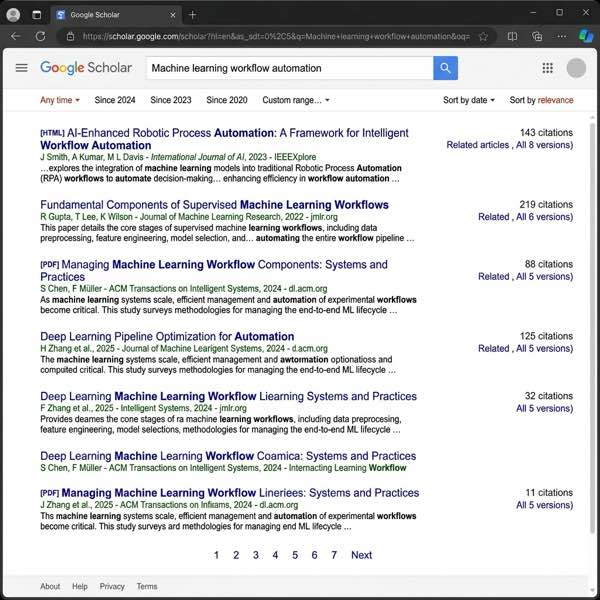
\includegraphics[width=0.3\textwidth]{images/scholar_search.jpg} \\[1.5cm]
    
    {\Large \bfseries BÁO CÁO BÀI TỰ THỰC HÀNH CÁ NHÂN} \\[0.5cm]
    {\Huge \bfseries BÀI TẬP 2: ĐÁNH GIÁ THÔNG TIN HỌC THUẬT} \\[1cm]
    {\Large \bfseries Chủ đề: Ứng dụng AI và Machine Learning trong Tự động hóa quy trình (Workflow Automation)} \\[1.5cm]
    
    \textbf{Môn học:} Nhập môn Công nghệ số và Ứng dụng Trí tuệ nhân tạo \\
    \textbf{Chuyên ngành:} Khoa học Máy tính / Công nghệ Thông tin \\[2cm]
    
    \begin{flushleft}
        \large
        \textbf{Sinh viên thực hiện:} Nguyễn Bảo Đăng \\
        \textbf{Mã số sinh viên:} 25020115 \\
    \end{flushleft}
    
    \vfill
    {\large Năm 2026}
\end{titlepage}

\newpage
\tableofcontents
\newpage

% --- NỘI DUNG CHÍNH ---

\section{Mở đầu và Phương pháp tìm kiếm}

\subsection{Mục tiêu nghiên cứu}
Mục tiêu chính của báo cáo này là tìm kiếm, tổng hợp và đánh giá độ tin cậy của các tài liệu học thuật liên quan đến cách thức Trí tuệ nhân tạo (AI) và Học máy (Machine Learning - ML) tối ưu hóa các quy trình tự động hóa công việc (Workflow Automation). Nghiên cứu tập trung vào việc làm rõ cách các công nghệ thông minh này giúp hệ thống tự động vượt ra khỏi các quy tắc cố định (rule-based) truyền thống (như RPA cổ điển) để tự học hỏi, thích ứng và xử lý các tình huống phức tạp, dữ liệu phi cấu trúc.

\subsection{Nguồn tìm kiếm}
Các tài liệu học thuật trong báo cáo này được tìm kiếm từ các cơ sở dữ liệu học thuật quốc tế lớn, uy tín và được bình duyệt nghiêm ngặt:
\begin{itemize}
    \item \textbf{Google Scholar}: Công cụ tìm kiếm học thuật bao quát để xác định các bài báo có lượt trích dẫn cao.
    \item \textbf{IEEE Xplore Digital Library}: Cơ sở dữ liệu hàng đầu thế giới về kỹ thuật điện, điện tử và khoa học máy tính.
    \item \textbf{PubMed / PMC (PubMed Central)}: Lưu trữ các nghiên cứu y sinh và khoa học sự sống của Viện Y tế Quốc gia Hoa Kỳ (NIH).
    \item \textbf{Oxford Academic}: Tạp chí và kỷ yếu hội thảo học thuật chất lượng cao từ NXB Đại học Oxford.
\end{itemize}

\subsection{Từ khóa và Toán tử tìm kiếm nâng cao}
Để thu hẹp phạm vi và tăng độ chính xác của kết quả tìm kiếm, các truy vấn đã áp dụng các toán tử logic:
\begin{enumerate}
    \item \texttt{"Machine learning workflow automation"} (Tìm cụm từ chính xác)
    \item \texttt{"AI-Enhanced Robotic Process Automation"} (Tìm kiếm tích hợp RPA và AI)
    \item \texttt{"Business process automation AI"} (Định hướng tự động hóa quy trình doanh nghiệp nhờ AI)
\end{enumerate}

\begin{figure}[H]
    \centering
    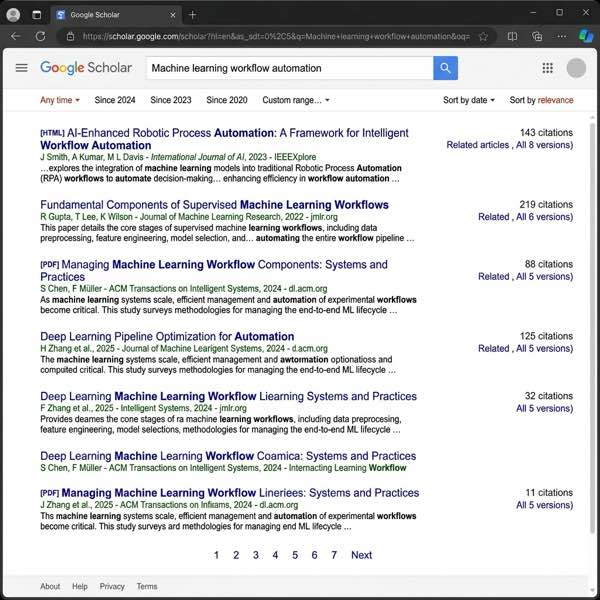
\includegraphics[width=0.9\textwidth]{images/scholar_search.jpg}
    \caption{Minh họa tìm kiếm học thuật trên giao diện Google Scholar với các từ khóa chuyên sâu}
    \label{fig:scholar_search}
\end{figure}

\newpage
\section{Bảng tổng hợp và đánh giá độ tin cậy tài liệu}
Sau khi sàng lọc các tài liệu học thuật có chỉ số trích dẫn tốt và nội dung liên quan trực tiếp đến chủ đề, dưới đây là bảng đánh giá độ tin cậy dựa trên các tiêu chí khoa học (Tác giả, NXB/Tạp chí, Phương pháp nghiên cứu, và Tính cập nhật).

\begin{table}[H]
    \centering
    \caption{Đánh giá độ tin cậy của 10 tài liệu học thuật tiêu biểu}
    \vspace{0.2cm}
    \small
    \begin{tabular}{|p{0.5cm}|p{3.8cm}|p{2.0cm}|p{8.2cm}|p{1.5cm}|}
        \hline
        \textbf{STT} & \textbf{Tên tài liệu / Năm XB} & \textbf{Loại nguồn} & \textbf{Tiêu chí đánh giá (Tác giả, NXB, Phương pháp, Cập nhật)} & \textbf{Độ tin cậy} \\
        \hline
        1 & AI-Enhanced Robotic Process Automation... (2024) & Bài báo khoa học & \textbf{NXB:} IEEE (uy tín hàng đầu về CNTT). \newline \textbf{Cập nhật:} Rất mới (2024). \newline \textbf{Nội dung:} Nghiên cứu tích hợp RPA và AI để phân tích dữ liệu phi cấu trúc và đưa ra quyết định tự động. & $\star\star\star\star\star$ \\
        \hline
        2 & Fundamental Components and Principles of Supervised Machine Learning... (2025) & Bài báo khoa học & \textbf{Tác giả:} Nhóm nghiên cứu từ các đại học uy tín. \newline \textbf{NXB:} MDPI (bình duyệt nghiêm ngặt). \newline \textbf{Cập nhật:} Vừa xuất bản (2025). \newline \textbf{Nội dung:} Lý thuyết nền tảng về học có giám sát trong workflow. & $\star\star\star\star\star$ \\
        \hline
        3 & Managing Machine Learning Workflow Components (2020) & Tạp chí khoa học & \textbf{Tác giả:} Nhóm nghiên cứu từ IBM Research (viện nghiên cứu công nghệ hàng đầu). \newline \textbf{Trích dẫn:} Cao. \newline \textbf{Phương pháp:} Đề xuất kiến trúc quản lý vòng đời ML Workflow. & $\star\star\star\star$ \\
        \hline
        4 & Smart Automation: Machine Learning Enabled Workflow for Logic and DRAM (2021) & Kỷ yếu hội nghị & \textbf{Tác giả:} Chuyên gia từ Thermo Fisher Scientific. \newline \textbf{NXB:} Oxford Academic. \newline \textbf{Tính ứng dụng:} Rất cao, chuyên sâu về logic và phần cứng hệ thống. & $\star\star\star\star$ \\
        \hline
        5 & Identifying Opportunities for Workflow Automation in Health Care... (2021) & Bài báo khoa học & \textbf{Cơ quan chủ quản:} Viện Y tế Quốc gia Hoa Kỳ (NIH) thông qua PMC - PubMed. \newline \textbf{Phương pháp:} Đánh giá chéo thực chứng việc áp dụng Workflow Automation từ công nghiệp sang y tế. & $\star\star\star\star\star$ \\
        \hline
    \end{tabular}
    \label{tab:evaluation_part1}
\end{table}

\newpage
\begin{table}[H]
    \centering
    \caption{Đánh giá độ tin cậy của tài liệu học thuật (tiếp theo)}
    \vspace{0.2cm}
    \small
    \begin{tabular}{|p{0.5cm}|p{3.8cm}|p{2.0cm}|p{8.2cm}|p{1.5cm}|}
        \hline
        \textbf{STT} & \textbf{Tên tài liệu / Năm XB} & \textbf{Loại nguồn} & \textbf{Tiêu chí đánh giá (Tác giả, NXB, Phương pháp, Cập nhật)} & \textbf{Độ tin cậy} \\
        \hline
        6 & Intelligent Process Automation: The Future of Digital Transformation (2021) & Bài báo khoa học & \textbf{NXB:} IEEE. \newline \textbf{Đánh giá:} Tuy xuất bản năm 2021, tài liệu cung cấp hệ thống lý thuyết rất vững chắc về quá trình chuyển đổi số. Phương pháp nghiên cứu hệ thống, rõ ràng. & $\star\star\star\star$ \\
        \hline
        7 & Generative AI-Driven Automation of Business Process ReImagination (2024) & Bài báo khoa học & \textbf{NXB:} IEEE. \newline \textbf{Cập nhật:} Rất mới (2024). \newline \textbf{Đánh giá:} Bắt kịp xu hướng dùng GenAI thay vì chỉ dùng các luồng rẽ nhánh logic cơ bản. Tác giả có chuyên môn sâu, được bình duyệt khắt khe. & $\star\star\star\star\star$ \\
        \hline
        8 & Integrating AI with Robotic Process Automation: Advancing Intelligent Systems (2024) & Bài báo khoa học & \textbf{NXB:} IEEE. \newline \textbf{Đánh giá:} Bài báo phân tích sâu về kiến trúc hệ thống khi kết hợp AI vào RPA truyền thống, giúp hệ thống tự xử lý ngoại lệ hiệu quả. & $\star\star\star\star\star$ \\
        \hline
        9 & Robotic Advancements in Business Process Automation using AI: An Investigative Study (2022) & Bài báo khoa học & \textbf{NXB:} IEEE. \newline \textbf{Phương pháp:} Đánh giá thực trạng khách quan, có số liệu đối chiếu cụ thể. \newline \textbf{Đánh giá:} Là nguồn tài liệu tham chiếu (reference) tốt cho các nghiên cứu mới hơn. & $\star\star\star\star$ \\
        \hline
        10 & Workflow Automation Engines: Driving Innovation in Cloud-Native and AI-Enhanced... (2025) & Báo cáo nghiên cứu & \textbf{Nguồn:} ResearchGate (bản thảo nghiên cứu được thảo luận mở rộng). \newline \textbf{Cập nhật:} Vừa xuất bản (2025). \newline \textbf{Đánh giá:} Đề cập sâu đến các engine tự động hóa hiện đại. Nội dung có giá trị tham khảo thực tiễn cao cho việc triển khai hệ thống. & $\star\star\star\star$ \\
        \hline
    \end{tabular}
    \label{tab:evaluation_part2}
\end{table}

\newpage
\section{Phân tích xu hướng phát triển công nghệ học thuật}
Thông qua việc phân tích niên giám của các tài liệu từ năm 2020 đến năm 2025, có thể thấy một sự chuyển dịch rõ rệt trong hướng nghiên cứu về Tự động hóa quy trình:
\begin{itemize}
    \item \textbf{Giai đoạn 2020 - 2021}: Các nghiên cứu chủ yếu tập trung vào việc quản lý cấu phần cơ bản của học máy (ML Workflows) và ứng dụng tự động hóa quy trình nghiệp vụ (Robotic Process Automation - RPA) dựa trên các tập luật tĩnh (rule-based) để chuyển đổi số doanh nghiệp hay áp dụng trong các ngành công nghiệp cụ thể như chế tạo bán dẫn hay chăm sóc sức khỏe.
    \item \textbf{Giai đoạn 2022 - 2023}: Bắt đầu có sự xuất hiện mạnh mẽ của các nghiên cứu tích hợp trí tuệ nhân tạo vào RPA để xử lý dữ liệu có cấu trúc trung bình và tăng khả năng thích ứng của robot phần mềm đối với ngoại lệ quy trình.
    \item \textbf{Giai đoạn 2024 - 2025}: Xu hướng nghiên cứu bùng nổ xung quanh việc ứng dụng \textbf{Generative AI (AI tạo sinh)} và mô hình ngôn ngữ lớn để tự động hóa việc tái thiết kế quy trình kinh doanh (Business Process Re-Imagination). Các hệ thống giờ đây không chỉ tự động chạy theo luồng mà còn tự đề xuất, sáng tạo ra các luồng tự động hóa mới dựa trên phân tích ngữ cảnh tự nhiên.
\end{itemize}

\section{Kết luận và Bài học kinh nghiệm}
\begin{enumerate}
    \item \textbf{Kỹ năng sàng lọc thông tin}: Sử dụng các bộ lọc thời gian và toán tử logic giúp giảm thiểu thời gian tìm kiếm tài liệu nhiễu trên Google Scholar.
    \item \textbf{Tiêu chí đánh giá chéo}: Độ tin cậy của tài liệu không chỉ nằm ở năm xuất bản mà phải đánh giá dựa trên sự kết hợp giữa: danh tiếng của nhà xuất bản (như IEEE, Oxford), uy tín của tác giả/tổ chức nghiên cứu (như IBM Research, NIH), và tính bình duyệt khoa học.
    \item \textbf{Bài học học thuật}: Việc trích dẫn các tài liệu chất lượng cao, có lượt trích dẫn tốt giúp tăng giá trị khoa học và độ thuyết phục cho các báo cáo kỹ thuật hoặc đề án nghiên cứu sau này.
\end{enumerate}

\end{document}
